\chapter{FlipIt with a virus propagation }
\label{cha:6}
%\documentclass[10pt]{article}\

%%%%%%%%%%%%%%%%%%%%%%%%%%%%%%%%%%%%%%%%%%%%%%%%%%%%%%%%%%
%%%%%			Introduction Chapter 6			%%%%%%
%%%%%												%%%%%%
%%%%%												%%%%%%
%%%%%%%%%%%%%%%%%%%%%%%%%%%%%%%%%%%%%%%%%%%%%%%%%%%%%%%%%%

\todo{resources vs nodes}
\section{Introduction}

%This section gives a formal definition of the FlipIt game with a virus propagation. First we derive a formula for a FlipIt game without a virus. After that we introduce a modification to this formula to achieve an adapted formula for a FlipIt game with a virus propagation. 
In this section we are going to elaborate how we are going to model a FlipIt game with multiple resources and a virus that propagates and infects the resources. First we derive a formula for a FlipIt game without a virus. After that we introduce a modification to this formula to achieve an adapted formula for a FlipIt game with a virus propagation. 
% We come up with a formula for the normal FlipIt (normal as in specific parameters and no normalising over the first interval) and then reform it to a FlipIt game with a virus. 

\subsection{FlipIt vs FlipIt with virus propagation}
Section [] explained the FlipIt game. This section will adapt a FlipIt game to a FlipIt game with virus propagation. We consider the non-adaptive continuous FlipIt game where both players play a periodic strategy with a random phase. De adaptation will be a game where the single resource consist of a computer network with multiple nodes. One of the players, the defender, will try to defend his network. The defender will do this by flipping all the nodes of the network in every move he plays. The attacker, the other player, will try to infect all the nodes in the network. The attacker will do this by flipping the node in the graph that can infect all the nodes in the shortest time possible. The attacker will only gain the control over the resource when he infects all the nodes of the network. The defender in contrast will gain control over the whole network when it has control over at least one node in the network. \\
\todo{ergens vermelden waarom we deze case bespreken en niet waarbij de aanvaller niet periodisch speelt}

After dropping a virus on the first resource, it takes a while for the virus to infect the entire network. The time that it takes for the virus to infect every node will be denoted as parameter \textit{d}. If we want to measure how long it takes for the virus to infect all the nodes in the network, we have to calculate the shortest path from the first infected node to the farthest node. This can be measured by a method that we will explain in section []. Using this parameter, a FlipIt game with virus propagation can be modelled. \\ 




%If the attacker attacks with the virus, the propagation will cause a delay of length \textit{d} before the attacker gains control over the whole network. This means that the gain of the attacker from the normal game has to be substracted with a delay every time the attacker moves. This game, where the attacker drops a virus, cannot be modelled completely by a FlipIt game with a delay. It may happen that the delay \textit{d} is bigger than the initial amount of control of the attacker. In this case the attacker will gain no control. If it would be with the delay caused by a phase bigger than zero the attacker would gain control after the defender flipt again. This is explained in figure \ref{fig:virusflip}. In the next section a formal definition .. \todo{verder uitleggen nog. Phases zijn vooraf uitgelegd.}




\subsection{define formula}
%The game FlipIt with a virus propagation is a two-player game with multiple resources. The multiple resources represent the nodes in a network. One of the players, the defender, will try to defend his network. The defender will do this by flipping all the nodes of the network in every move he plays. The attacker, the other player, will try to infect all the nodes in the network. The attacker will do this by flipping the node in the graph that can infect all the nodes in the shortest time possible. The attacker will gain the control over the network when all the resources are infected. So parameter \textit{d} will be the time of the shortest path from the start node to the furthest node. \\


\todo{deze sectie herschrijven}
There is a definition given for the gain of a player \textit{i} by the writers of the paper FlipIt [], but we want to add the property of a virus propagation to the game, hence parameter \textit{d}, so we are trying to find another formula that defines a game by counting the amount of time one of the players has control. \\
\todo{we hebben een periodisch spel, simpelste spel.}


\todo{zeggen dat we eerst de functie voorstellen van de normale FlipIt}
First a list of notations that will be used throughout the formal definition (see figure \ref{fig:notations} for a graphic representation of some of the notations):
\begin{description}
\item $\delta_{0}$: Positive and non zero number. This is the period of the defender. This denotes the length of the interval between two consecutive moves of the defender. 
\item $\delta_{1}$: This is the period of the attacker. This denotes the length of the interval between two consecutive moves of the attacker.
\item \textit{$T_{0}$}: This denotes the phase of the defender that was random and uniform chosen over the interval [0,$\delta_{0}$].
\item \textit{$T_{1}$}: This denotes the phase of the attacker that was chosen uniformly at random in interval [0,$\delta_{1}$].
\item \textit{Unit of control}: Defined as the period between gaining control and losing control over the resource.  
\item \textit{n}: n is the n'th interval of the attacker, starting from interval 1.
\item $\Delta A$ : This is a function that denotes the length of a unit of control of the attacker in the n'th interval of the attacker.
\item \textit{d}: Amount of time that the virus needs to infect every node in the network.
\item \textit{lcm(a,b)}: The \textit{lcm} of a and b is the least common multiple of a and b.
\item \textit{gcd(a,b)}: The \textit{gcd} of a and b is the greatest common divider of a and b.
\item \textit{Gain}:  The gain of a player is defined as the total amount of time that a player has owned the resource since the start of the game. In the context of a FlipIt game with virus propagation, the whole network is seen as one resource. This resource is owned by the attacked if he has control over the entire network. If the defender owns at least one node, he owns the resource.\\
\item \textit{Average Gain}:  $\gamma_{i}(t) = G_{i}(t)/t$ is the average gain rate of player \textit{i} which is defined as the fraction of time that player \textit{i} has control over the resource up to time t.
\item \textit{Benefit}: The average benefit of a player \textit{i} is denoted by $\beta_{i}(t) = \gamma_{i}(t) - k_{i} / \delta_{i}$, which is equal to the fraction of time that the resource has been owned by player \textit{i}, minus the cost rate for moving. For now we consider the cost rate equal to 0. In the rest of the paper the average benefit will be addressed as the benefit of the game for player \textit{i}.
\end{description}
\begin{figure}[hbtp]
\caption{Defining unit of control}
\centering
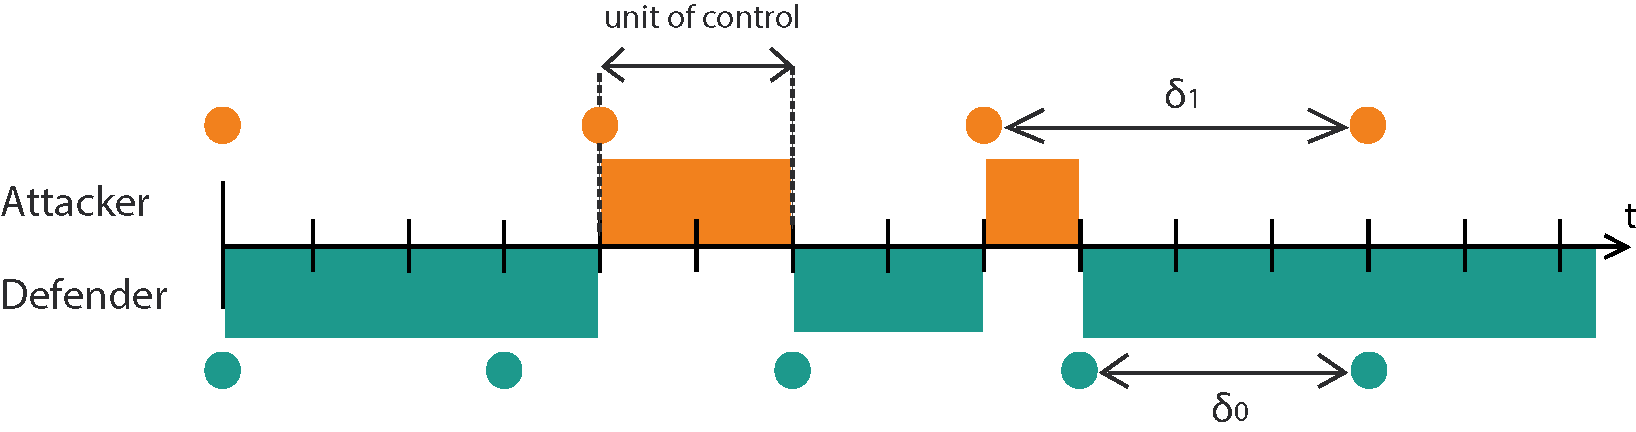
\includegraphics[scale=1]{Images/FlipSpel.png}
\label{fig:notations}
\end{figure}


%\begin{equation}\label{first}
%n = \delta_{1} mod \delta_{0}
%\end{equation}
%
%\begin{equation}\label{first}
%\Delta A = [( \delta_{0} - n + 1 ) * \delta_{1}] mod \delta_{1}
%\end{equation}
%
%\begin{equation}\label{first}
%\sum_{i=0}^{\delta_{1}} \lbrace [( \delta_{0} - i + 1 ) * \delta_{1}] mod \delta_{1} \rbrace
%\end{equation}
%\todo{formule met i nakijken}


\todo{We mag gebruikt worden in een wetenschappelijke tekst zolang de focus blijft op het werk en niet op de schrijver, FlipIt schrijvers gebruiken ook veel de we vorm} 
We start by computing the gain of the attacker in a periodic game without phases. Two cases are considered: case 1 where the defender moves as least as fast as the attacker and case 2 where the attacker plays as least as fast as the defender. After that we introduce the phases. Next we adapt our gain calculation to include virus propagation. Finally we compute the benefit of the attacker in function of the gain.   
\\
\subsubsection{Computing the gain for an attacker of a normal FlipIt game}
\textbf{Case  1:} \\
For $\delta_{1} > \delta_{0}$ (The defender moves faster than the attacker.) \\

We consider a game in which both of the players start with a phase $T_{0}$ and phase $T_{1}$ equal to zero. Both players start their first move at $t=0$. As previously stated (in the formal definition of the game and the introduction of different notations used throughout the paper), the defender has control in the beginning of the game at $t=0$. If the two players move at the same time during the game, the moves cancel and no change of state happens. \\ \todo{eerder gedefinieerd dat elk spel begint op t=0}

To compute the gain formula for the attacker, we need to calculate the amount of time that the attacker has control over the game from the start of the game up to time t. This can be done by computing all the units of control of the attacker up to time t \todo{formule is niet in staat om dat te doen als functie van t} and summing them. \\
The formula that we are going to compute will not be in function of the time but in function of the intervals of the attacker. By doing this we always have a whole unit of control. If time is used the last unit of control can be shortened. Because the game goes on indefinitely and because it is easier to compute a formula in function of the intervals of the attacker, the gain formula will be in function of the intervals of the attacker. \todo{kan misschien beter uitgelegd worden}

For that reason we divide our time line of our FlipIt game into different intervals of size $\delta_{1}$. Therefore every time the attacker moves we have the start of a new interval. Considering that the defender will move faster than the attacker, he or she will at least move one time during the interval of the attacker. Because the attacker only moves at the start of his or her interval we can say that the defender will always end as being in control of the resource. \todo{tekening met voorbeeld}. To calculate how long the unit of control of the attacker is in the n'th interval, we only need to know how long the attacker has control over the resource before the defender moves in that interval. First we need to calculate the start time of the n'th interval which will be a multiple of the period of the attacker. Once we know this we need to know what the difference is between this amount of time and the amount of time when the defender will flip. To do this we take the modulo of the negative of the amount of time of the attacker with the period of the defender. By doing so we calculate how much it takes to add to this time to compleet to a time that is a multiplier of the period of the defender. See figure \ref{fig:modulo} to see a graphic representation of this modulo. 
\todo{blabla en dan hebben we de volgende formule}
\begin{figure}[hbtp]
\caption{Taking the modulo of a negative number}
\centering
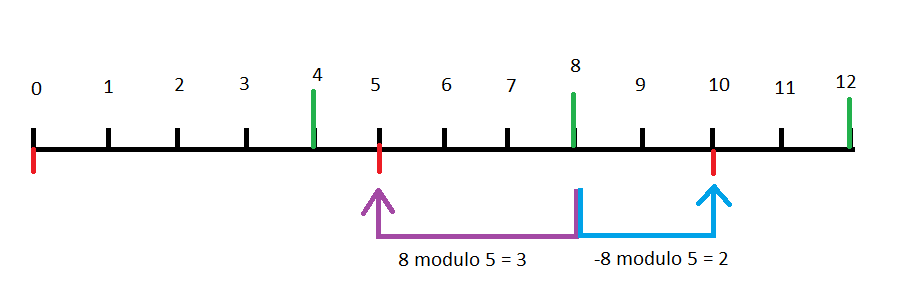
\includegraphics[scale=0.6]{Images/Modulo.png}
\label{fig:modulo}
\end{figure}

\todo{modulo uitleggen en dan verder door tot deze formule}
This brings us to the next forumula to calculate the length of a unit of control in the n'th interval of the attacker. 
\todo{definieer dat delta groter als nul is en niet negatief}
For every positive and non zero real $\delta_{1}$ and $\delta_{0}$ $\in$ \(\mathbb{R}\) and every n $\in$ \(\mathbb{N}\) (including 0 in the set of natural numbers) :
\begin{equation}\label{first}
\Delta A = [( 1- n  ) \cdot \delta_{1}] mod \delta_{0}
\end{equation}
where n is the number of the n'th interval of the attacker where the length of the unit of control of the attacker is calculated.\\

%In this formula we multiply the number of unit of control that we want with the period of Attacker ( $\delta_{1}$). 
The 1 - n is when we count beginning from 1. If we start counting starting at 0 we leave the 1 and the formula becomes:
\begin{equation}\label{first}
\Delta A = [( - n  ) \cdot \delta_{1}] mod \delta_{0}
\end{equation}

An example: Figure \ref{fig:modulo} shows a FlipIt game were the period of the attacker is Pi and the period of the defender is 1. .. voorbeeld klopt.
On figure \ref{fig:unitofcontrolformula} 
\begin{figure}[hbtp]
\caption{Example for calculating the control unit in interval 3 for a FlipIt game with period defender = 1 and period attacker = Pi}
\centering
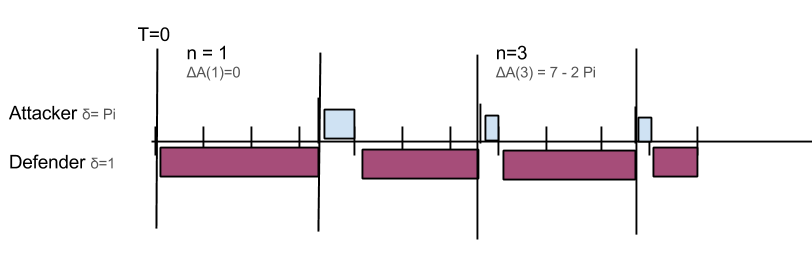
\includegraphics[scale=0.6]{Images/VoorbeeldUnit.png}
\label{fig:unitofcontrolformula}
\end{figure}

%We know that each interval ends with the control for the defender. This means that we only need to know how long the defender had control during that interval and take the rest. The rest will be the amount of time the attacker has control in that interval. We take the rest by doing the $mod \delta_{0} $

For phases .. \\

\textbf{Case 2}:
Alles omdraaien \todo{beter beschrijven}



\subsection{Formula with a virus propagation}
Now we can define how we can use the previous formula to calculate the gain of the attacker in a FlipIt game with virus propagation.
As mentioned before parameter \textit{d} defines the virus propagation. It will take an amount of time \textit{d} before the attacker gains control over all the resources. In the previous section we defined a formula to calculate each unit of control of the attacker. If the virus propagation takes \textit{d} time before every resource is infected then this d has to be subtracted from each unit of control. (see figure \ref{fig:virusflip}). It may happen that the unit of control is less than \textit{d}. The result of the substration will be a negative number in time. In this case this means that the defender has flipped all the resources before the attacker could gain control over all the resources. To calculate the gain only the units of control bigger than 0 have to be summarized. So the formula becomes:

\begin{equation}\label{first}
Gain_{1} = \sum_{i=0}^{\delta_{0}} \lbrace [( 1 - i ) \cdot \delta_{1}] mod \delta_{0} - d \rbrace  > 0 \rbrace 
\end{equation}

\begin{figure}[hbtp]
\caption{Difference in a FlipIt game between delay caused by a virus and a phase bigger than zero for the Attacker}
\centering
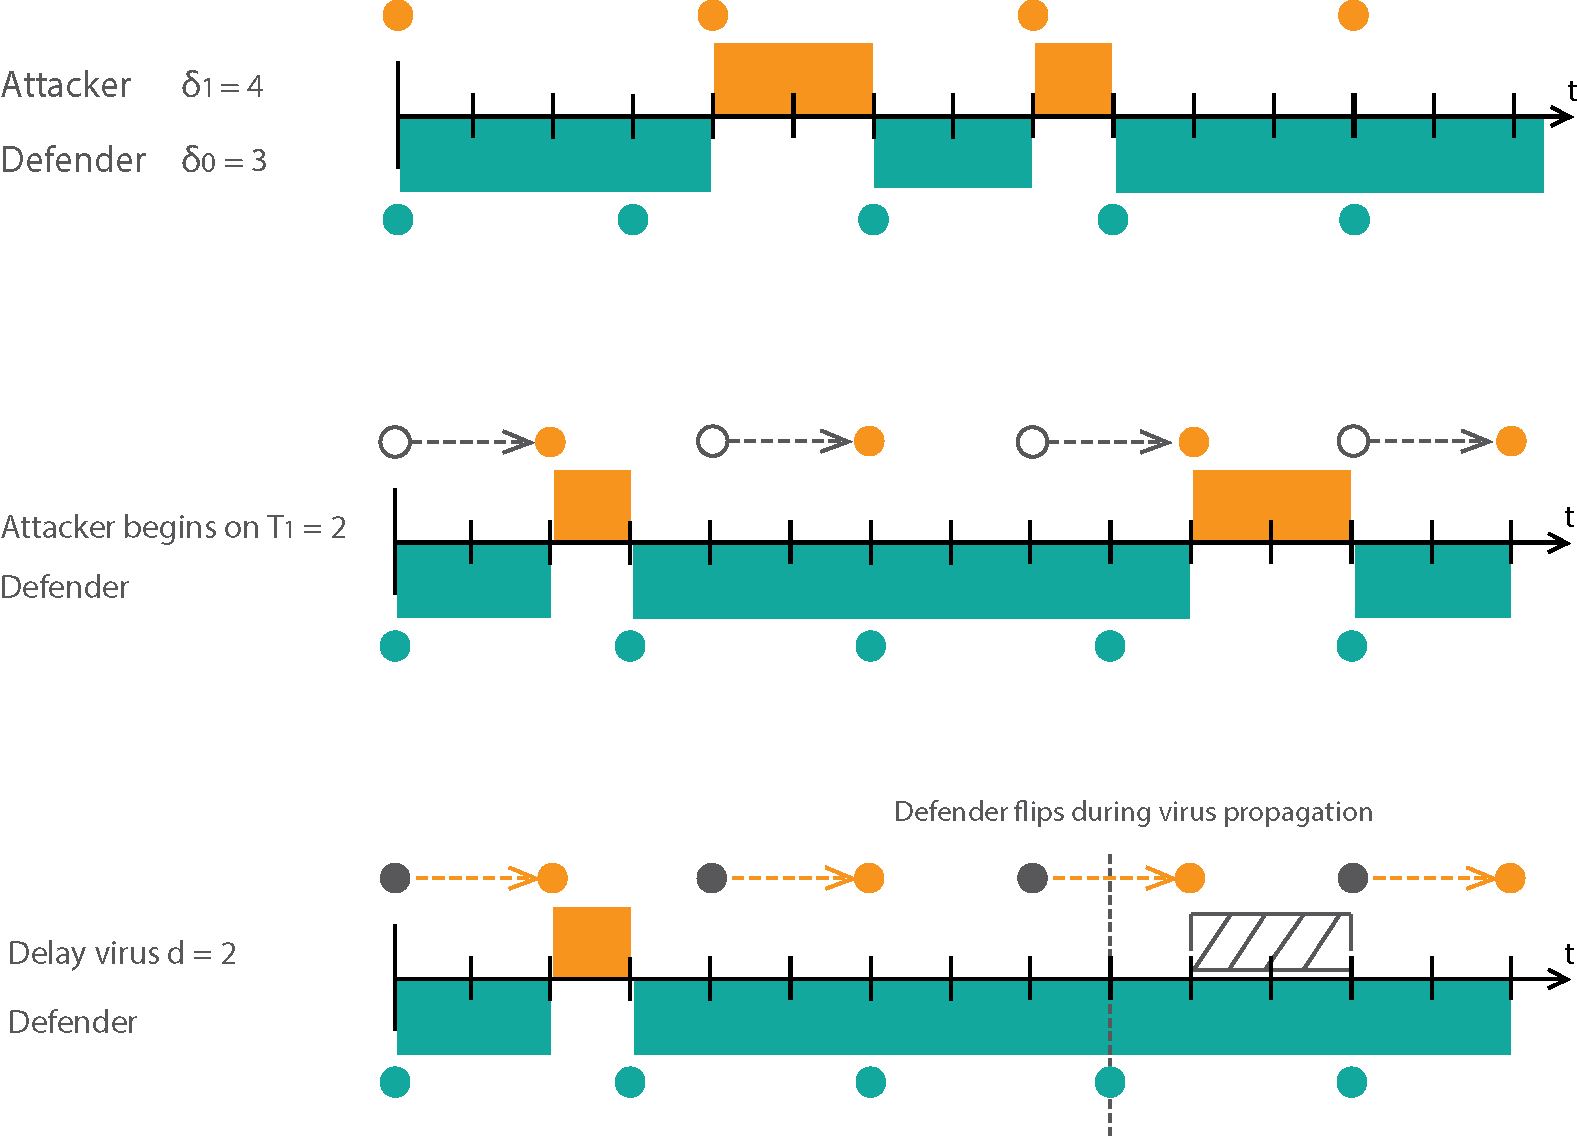
\includegraphics[scale=1]{Images/Flipvirus}
\label{fig:virusflip}
\end{figure}


\subsubsection{Computing the benefit of a FLipIt game with virus propagation}

To be able to calculate the benefit of the attacker, we need to calculate the average gain rate of the attacker. We will look at this for two cases. One case where $\delta_{0}$ and $\delta_{1}$ $\in$ \(\mathbb{Q}\) and the other one where $\delta_{0}$ and $\delta_{1}$ $\in$ \(\mathbb{I}.\) \\

\textbf{Rational numbers (\(\mathbb{Q}\)):} For $\delta_{0}$ and $\delta_{1}$ $\in$ \(\mathbb{Q}\), a repetition of the game will occur. As every rational number is any number that can be expressed as the fraction p/q with p and q $\in$ \(\mathbb{Z}\) (integers), with the denominator q not equal to zero, it is possible to find the \textit{lcm} of $\delta_{0}$ and $\delta_{1}$. The \textit{lcm} is defined for all rational numbers as: $lcm(\dfrac{a}{b},\dfrac{c}{d})= \dfrac{a \cdot c}{gcd(b,d)} with  $ [\todo{referentie}]. When \textit{t} is equal to the \textit{lcm} of $\delta_{0}$ and $\delta_{1}$, both players will move again at the same time and this can be mapped to the beginning of the game. Because we stated that at the end of the interval of the attacker, the defender is in control and because if two players move at the same time the moves are cancelled, we can map this to the beginning of the game. Since the game goes on infinite, to calculate the average gain of the attacker, it is sufficient to calculate the average gain of the attacker only during this repetition equal to the \textit{lcm} of $\delta_{0}$ and $\delta_{1}$. 
%This means that if we want to calculate the gain of the attacker we need to calculate the time the attacker has control over the total amount of time that has passed by.
%For $\delta_{0}$ and $\delta_{1}$ $\in$ \(\mathbb{Q}\) we can see that we have a cycle. A pattern that comes back over and over again. That is when the amount of time is a multiple of $\delta_{0}$ and $\delta_{1}$ or the largest common multiplier (\textit{lcm}). At this point the Attacker and the Defender move at the same time what brings us back to the beginning.
So to calculate the gain of $\delta_{0}$ and $\delta_{1}$ $\in$ \(\mathbb{Q}\) we need to calculate the amount of control units of the attacker that go into the length of time units equal to the \textit{lcm} of  $\delta_{0}$ and $\delta_{1}$. This will be equal to the amount of time that the period of the attacker goes into the \textit{lcm}. We denote this by parameter \textit{p} and define it as follow:
\begin{equation}\label{first}
p = \dfrac{lcm(\delta_{0},\delta_{1})}{\delta_{1} } 
\end{equation}
After this calculation we summarize our units of control in function of \textit{p} and divide it by the \textit{lcm} of $\delta_{0} $ and $ \delta_{1}$, which is the total amount of time for one cycle.  This gives us the following formula of the benefit of the attacker with a cost rate equal to zero:

\begin{equation}\label{first}
\beta_{1} = \dfrac{\sum_{i=0}^{p} \lbrace [( 1 - i ) \cdot \delta_{1}] mod \delta_{0} \rbrace }{lcm(\delta_{0},\delta_{1})} 
\end{equation}

%We can also define a formula without the greatest common divider. Every $\delta_{0}$ and $\delta_{1}$ have to be written in a fraction:
%\begin{equation}\label{first}
%\delta_{0}=\dfrac{a}{b} ~~~~and~~~~\delta_{1}=\dfrac{c}{d}
%\end{equation}
%If  $\delta_{0}$ or $\delta_{1}$ is a Geheel getal then b or d will be 1. The formula for the gain becomes different:\\
%
%\todo{formule zoeken zonder lcm en gcd}


\textbf{Irrational numbers (\(\mathbb{I}\)):} If $\delta_{0}$ and/or $\delta_{1}$ $\in$ \(\mathbb{I}\):
An irrational number $ i \neq \dfrac{a}{b}$ with $b \in$ \(\mathbb{Z}\) , a $\in$ \(\mathbb{N}\).
Because we cannot write \textit{i} as a fraction, this means that we cannot compute a common multiplier of $\delta_{0}$ and $\delta_{1}$. If their is no common multiplier the attacker and the defender won't move at one point on the same time, meaning that this does not result in a cycle. If we would have a cycle that means that there exists a number \textit{x} that can be divided by $\delta_{0}$ and $\delta_{1}$. At $t=x$ both of the players will move at the same time, which is not possible because then their would be a cycle. Since their is no cycle it also means that no unit of control will be repeated two times. Every unit of control will have a distinct length. If it does that means that their is repetition, meaning again that their is a cycle. \todo{nog verder uitleggen} We can conclude that if we have no cycle and no number will be repeated twice, that it will enumerate every number between 0 and the biggest interval (which is $\delta_{0}$). 
\textit{The reals are uncountable; that is: while both the set of all natural numbers and the set of all real numbers are infinite sets, there can be no one-to-one function from the real numbers to the natural numbers} [WikiPedia: real numbers] If they are uncountable that means that we cannot calculate the sum of all the numbers between 0 and the biggest interval. This is proved by the Cantor diagonalisation argument. Uncountable does not mean that we cannot order it. The Field of the real numbers is ordered. 

What we can do is take the limit, count as many control units of time of the attacker and divide it by the greatest amount of time. We can see that this eventually will result to the solution given by the writers of FlipIt. [r/2]. Example delta1 Pi and delta0 1. Grafiek voor maken.

%\subsection{Random phase}
%For now we assumed that the first move of both players started at phase $t=0$. In the FlipIt game the first move is chosen uniformly over the interval [0,$\delta$]. We will call this first move the phase move and denote it by $T_{1}$ for the attacker and $T_{0}$ for the defender.
%We will have to integrate these two phases into the formula.  
%\begin{equation}      
%\boxed{\eta \leq C(\delta(\eta) +\Lambda_M(0,\delta))}
%\end{equation}
%
%\begin{equation}\label{first}
%a=b+c
%\end{equation}
%
%\begin{subequations}\label{grp}
%\begin{align}
%a&=b+c\label{second}\\
%d&=e+f+g\label{third}\\
%h&=i+j\label{fourth}
%\end{align}
%\end{subequations}



%%% Local Variables: 
%%% mode: latex
%%% TeX-master: "thesis"
%%% End: 


